
\section{MANV}

\begin{frame}{MANV}
	\begin{itemize}
		\item MANV: \alert{Massenanfall von Verletzten}
		\item Begriff aus dem Rettungswesen
		\item Tritt ein bei einem Ereignis mit vielen Verletzten
		\item Probleme:
		      \begin{itemize}
			      \item Koordination der Rettungskräfte
			      \item Verteilung von Ressourcen
			      \item Außergewöhnliche Situation auch für Rettungskräfte
		      \end{itemize}
	\end{itemize}
\end{frame}

\begin{frame}{MANV - Beispiele}
	\begin{figure}
		\begin{center}
			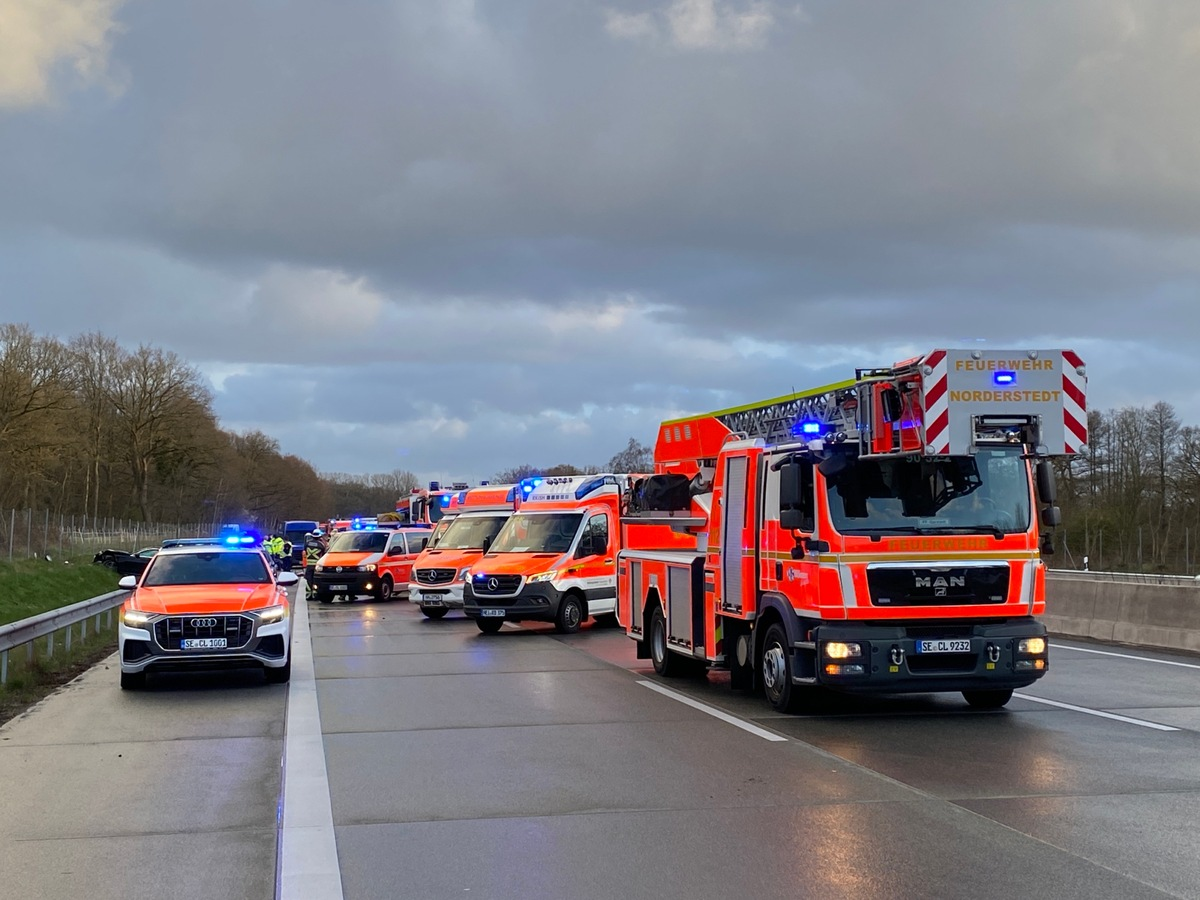
\includegraphics[width=0.4\textwidth]{images/autounfall.jpg}
		\end{center}
		\caption{Autounfall auf A7 zwischen Schnelsen-Nord und Quickborn mit 11 Betroffenen, davon einer tödlich verletzt.\cite{manv-a7}}\label{fig:autounfall}
	\end{figure}
\end{frame}

\begin{frame}{MANV - Beispiele}
	\begin{figure}
		\begin{center}
			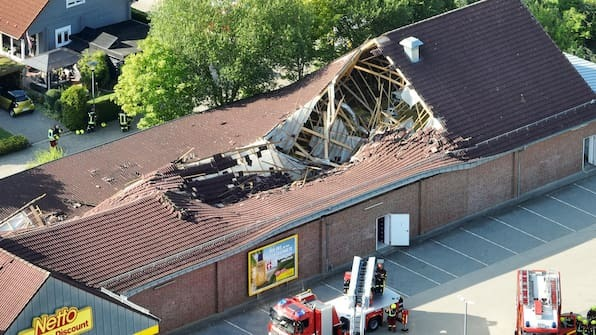
\includegraphics[width=0.5\textwidth]{images/ratzeburg-netto.jpg}
		\end{center}
		\caption{Dacheinsturz eines Supermarktes in Ratzeburg am 30.7.2024. 12 Leichtverletzte.\cite{manv-ratzeburg}}\label{fig:netto}
	\end{figure}
\end{frame}

\begin{frame}{MANV - Beispiele}
	\begin{figure}
		\begin{center}
			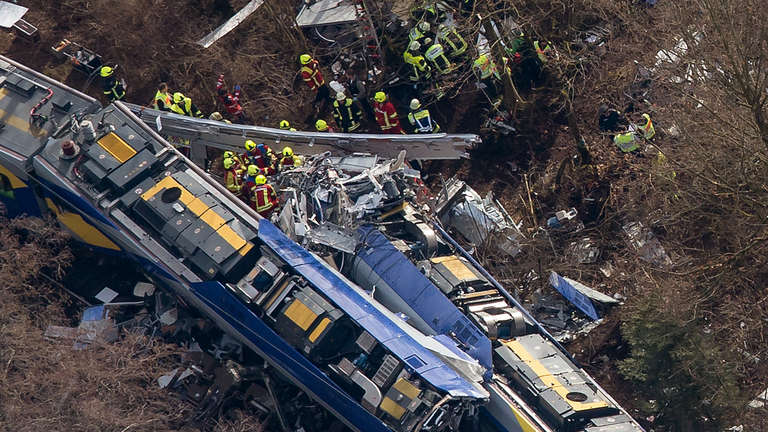
\includegraphics[width=0.5\textwidth]{images/bad-aibling.jpg}
		\end{center}
		\caption{Zugunglück von Bad Aibling. 12 Tote, 18 Schwerverletzte, 63 Leichtverletzte.\cite{manv-badaibling}}\label{fig:badaibling}
	\end{figure}
\end{frame}


\begin{frame}{MANV - Übung i}
	\begin{itemize}
		\item Vorbereitung auf den Ernstfall
		\item Regelmäßige Übungen
		\item Nicht standardisiert, jedoch Leitfaden vom DRK \cite{kreuz2016durchfuhrung}
		\item Mögliche Übungsformen:
		      \begin{itemize}
			      \item Von: Übung in Sporthalle mit Blättern als Patienten
			      \item Bis hinzu: Übung mit Mimen, überregionalen Einsatzkräften, Fahrzeugen, Gelände
		      \end{itemize}
		\item Ablauf auf Organisationsebene:
		      \begin{itemize}
			      \item Planung (Szenario, Übungsverlauf, ...)
			      \item Vorbereitung (Termin finden, Mimen anheuern, ...)
			      \item Durchführung
			      \item Direkte Nachbereitung mit allen Beteiligten, direktes Feedback
			      \item Spätere Nachbereitung mit Führungskräften zur Datenauswertung
		      \end{itemize}
	\end{itemize}

\end{frame}

\begin{frame}{MANV - Übung ii}
	\begin{columns}
		\begin{column}{0.7\textwidth}
			\begin{itemize}
				\item Ziel: Teilnehmer sollen lernen, dass\dots
				      \begin{itemize}
					      \item \dots es ein MANV-Konzept gibt und wie es aussieht
					      \item \dots Zeit kostbar ist
					      \item \dots es nicht mehr um individuelle Patientenversorgung geht
					      \item \dots Triage wichtig ist
				      \end{itemize}
			\end{itemize}
		\end{column}
		\begin{column}{0.3\textwidth}
			\begin{figure}
				\begin{center}
					\includegraphics[height=0.4\textheight]{images/übung.jpg}
				\end{center}
				\caption{Übung eines MANV.\cite{manv1übung}}\label{fig:übung}
			\end{figure}
		\end{column}
	\end{columns}
\end{frame}
